%!TEX root=../document.tex

\section{Installation und Konfiguration}
Der erste Schritt war es Jenkins zu installieren.

\subsection{Erstes Problem mit VM}

Bei der Installation ist mein erstes Problem aufgetreten, da ich dachte dass es einfacher wäre Jenkins in einer virtuellen Maschine laufen zu lassen. Dies bedeutet es wurde Jenkins installiert, was recht einfach lief dadurch dass Jenkins im apt-get Repository liegt, und die Konfiguration funktionierte dank Tutorial auch flüssig. Nun ist mir aufgefallen, voralleim beim Plugins installieren, dass die VM sehr langsam ist bzw. bei manchen Plugins garnicht funktioniert - noch dazu kommt dass ich das gesamte Git-Repository auf die virtuelle Maschine kopieren musste da Jenkins die Dateien lokal bezieht. Nach längerer Frustration bin ich schlussendlich auf Windows umgestiegen.

\subsection{Installation in Windows}
Die Installation in Windows läuft auch einfach ab, man installiert das \verb|.msi| file, öffnet \verb|localhost:8080| und geht den Installations-Wizard durch. Es wurden die richtigen Plugins angewählt bei der Erstkonfiguration (Außer Jenkins Violations da dieses erst im Dashboard installiert werden kann) und ein Admin user wurde angelegt:

\begin{minipage}{\linewidth}
	\centering
	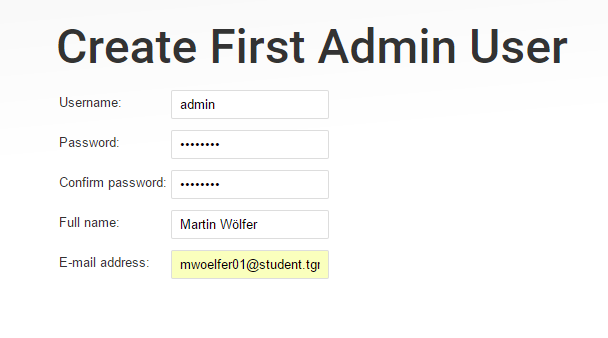
\includegraphics[width=0.8\linewidth]{images/create_admin}
	\figcaption{Ein Admin User wurde erstellt}
\end{minipage}

Anschließend wurde unter \verb|Manage Jenkins|  $\rightarrow$ \verb|Manage plugins| $\rightarrow$ \verb|Available| auch noch das letzte fehlende Plugin installiert (Jenkings Violations).

\subsection{Github-User Konfiguration}
Unter \verb|Manage Jenkins|  $\rightarrow$ \verb|Configure System| $\rightarrow$ \verb|Git Plugin| werden die Daten eingeben. 

\begin{minipage}{\linewidth}
	\centering
	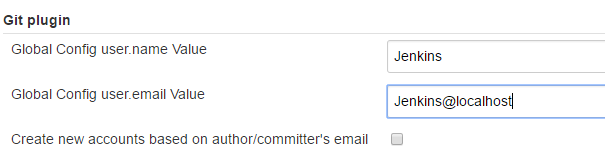
\includegraphics[width=0.8\linewidth]{images/git_plugin}
	\figcaption{Daten werden eingegeben für Git}
\end{minipage}

\section{Ersten Job erstellen}
Im Dashboard wird einem gleich angeboten einen Job zu erstellen, danach wird ein Name für den Job eingeben und es wird \verb|Freestyle Project| ausgewählt

\begin{minipage}{\linewidth}
	\centering
	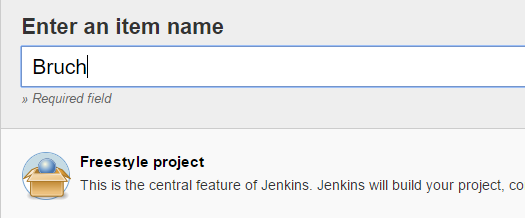
\includegraphics[width=0.8\linewidth]{images/new_job}
	\figcaption{Neuen Job erstellen}
\end{minipage}

\subsection{Job konfigurieren}
\subsubsection{Woher Job Quelle bezieht}
Zuerst muss Jenkins mitgeteilt werden wo die Quelle des Projektes überhaupt liegt, es wird zuerst unter der Section \verb|Source Code Management| der Button \verb|Git| angewählt, und anschließend der lokale Repository URL angegeben werden.

Hier bin ich auf ein weiteres Problem gestoßen, und zwar wurde die Fehlermeldung ausgeben: \textbf{jenkins failed to connect to repository}. Dies lag daran dass Jenkins nicht wusste wo sich lokal mein \verb|git.exe| befindet, daher musste ich in \verb|Manage Jenkins| $\rightarrow$ \verb|Global Tool Configuration| $\rightarrow$ \verb|Git| $\rightarrow$ \verb|Git Installations| den Pfad zu git.exe angeben:

\begin{minipage}{\linewidth}
	\centering
	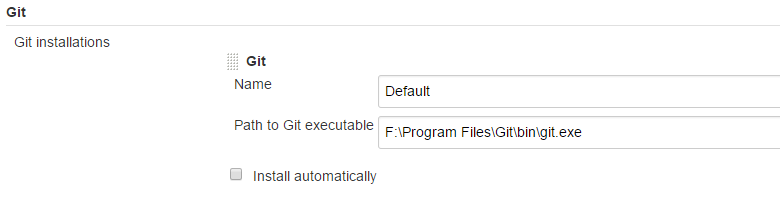
\includegraphics[width=0.6\linewidth]{images/path_to_git}
\end{minipage}

Nun konnte der lokale Pfad zum Repository angegeben werden ohne dass ein Problem besteht:

\begin{minipage}{\linewidth}
	\centering
	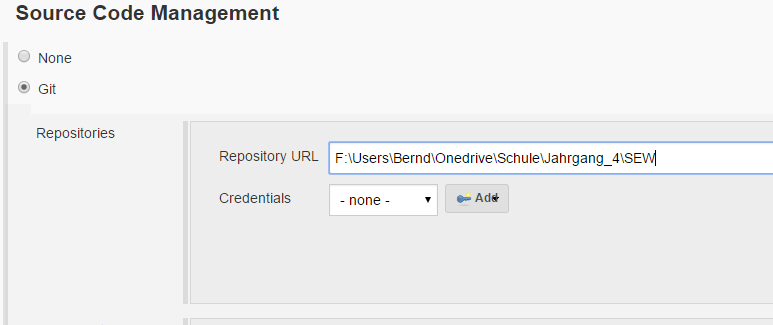
\includegraphics[width=0.8\linewidth]{images/path_to_repo}
	\figcaption{Pfad konnte angegeben werden ohne Fehlermeldung}
\end{minipage}

\subsubsection{Wann Job ausgeführt wird}
Nun wird unter \verb|Build Triggers| $\rightarrow$ \verb|Poll SCM| angegeben wann der Job ausgeführt wird, indem 5 \verb|*| angegeben werden:

\begin{minipage}{\linewidth}
	\centering
	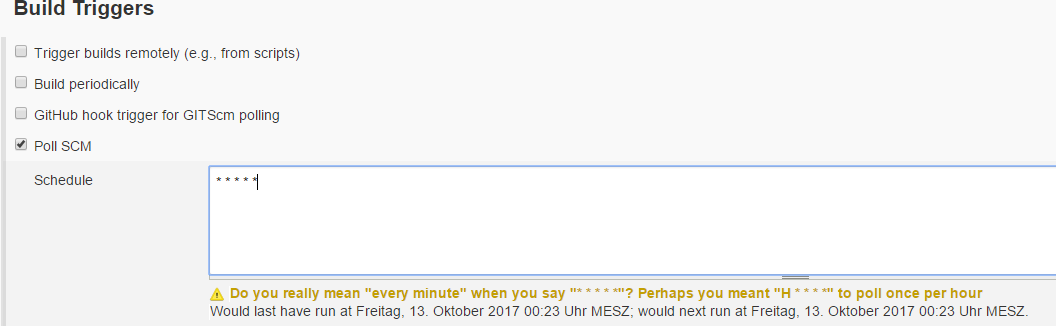
\includegraphics[width=0.8\linewidth]{images/build_triggers}
\end{minipage}

\subsubsection{Was ausgeführt wird}
Unter \verb|Build| $\rightarrow$ \verb|Add build step| $\rightarrow$ \verb|Execute Shell| wird nun folgender Code angegeben:

\begin{lstlisting}[language=bash]
nosetests --with-xunit --all-modules --traverse-namespace --with-coverage --cover-inclusive
coverage xml Testall.py 
pylint -f parseable -d I0011,R0801 testall.py > pylint.out | type pylint.out
\end{lstlisting}

Der erste Befehl erstellt das \verb|nosetests.xml| File. Es werden in dem momentanen Arbeitsfpad nach Tests gesucht, welche anschließend ausgeführt werden und in dem File gespeichert.

Der zweite command erstellt ein xml coverage report file vom File \verb|Testall.py|, in welchem alle Tests definiert sind.

Mit dem dritten Befehl wird das \verb|pylint.out| File erzeugt, in welchem violations erkannt werden. 

\subsubsection{Was passiert mit Ergebnissen}
In diesem Schritt wird nun entschieden wie die Ergebnisse analysiert werden. In diesem Fall werden sie interpretiert durch
\begin{itemize}
	\item Coverage
	\item JUnit testing
	\item Report Violations
\end{itemize}

Unter \verb|Post-build Actions| $\rightarrow$ \verb|Publish Cobertura Coverage Report| wird der Link zum Coverage File angegeben. Es wird lediglich \verb|coverage.xml| angegeben, weil dieses durch den Code im Schritt davor automatisch erzeugt wird.

\begin{minipage}{\linewidth}
	\centering
	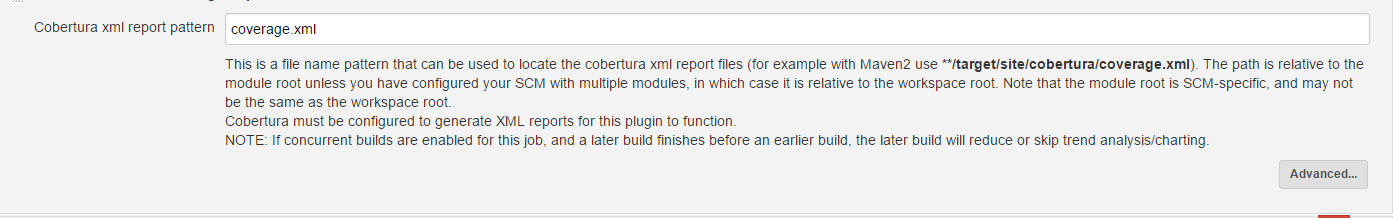
\includegraphics[width=0.8\linewidth]{images/coverage_report}
\end{minipage}

Als nächstes werden die JUnit Test results hinzugefügt. Dazu unter \verb|Post-build Actions| $\rightarrow$ \verb|Publish JUnit test result report| wieder den Filenamen angegeben vom Code erzeugten File, \verb|nosetest.xml|.

\begin{minipage}{\linewidth}
	\centering
	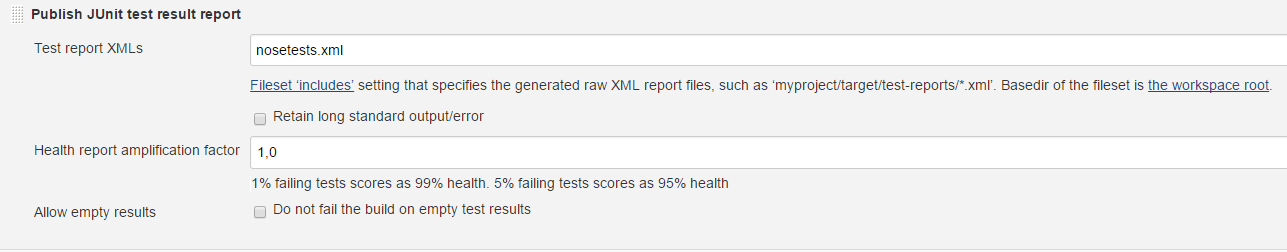
\includegraphics[width=0.8\linewidth]{images/junit_tests}
\end{minipage}

Der letzte Schritt ist es Report Violations zur Interpretation hinzuzufügen. Unter \verb|Post-build Actions| $\rightarrow$ \verb|Report Violations to GitHub| $\rightarrow$ \verb|PYLINT| im Feld \verb|Pattern| folgendes eingeben: \verb|**/pylint.out|. Dieses File wird auch durch den bereits erwähnten Code erstellt.

\begin{minipage}{\linewidth}
	\centering
	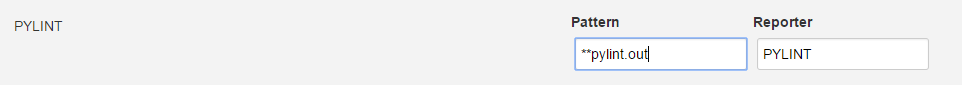
\includegraphics[width=0.8\linewidth]{images/report_violations}
\end{minipage}

Der Job muss nun nur mehr gespeichert werden.

\subsection{Job ausführen}
Dazu wird im Dashboard auf \verb|Build Now| gedrückt. Falls alles funktioniert sollte nun der Punkt Blau aufscheinen:

\begin{minipage}{\linewidth}
	\centering
	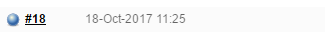
\includegraphics[width=0.5\linewidth]{images/run_job}
\end{minipage}

Man kann nun den Statusbericht einsehen, indem man auf den build drückt:

\begin{minipage}{\linewidth}
	\centering
	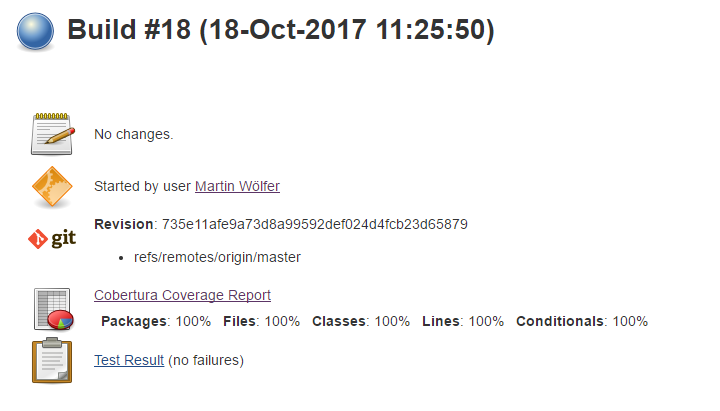
\includegraphics[width=0.8\linewidth]{images/status_report}
\end{minipage}

\subsubsection{Code Coverage}
Durch \verb|cobertura| kann das erstellte \verb|coverage.xml| file eingelesen werden und verarbeitet werden. Das Ergebnis sollte folgendermaßen aussehen:

\begin{minipage}{\linewidth}
	\centering
	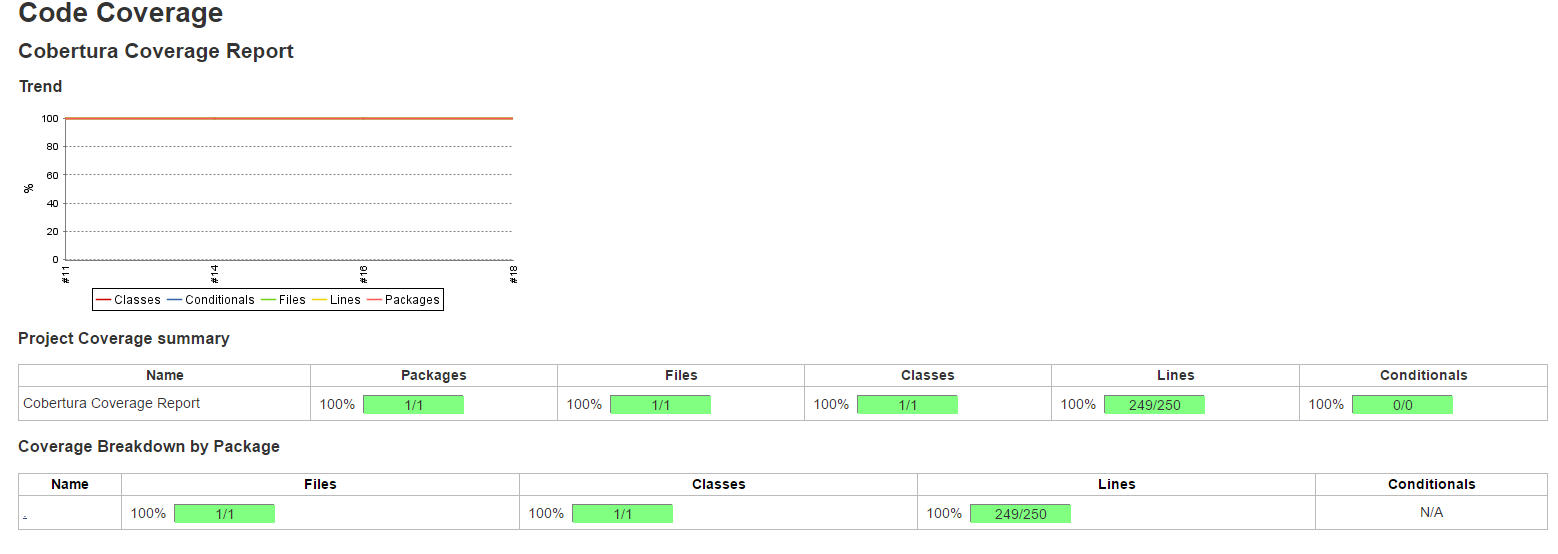
\includegraphics[width=1\linewidth]{images/coverage}
\end{minipage}

Man sieht nun das vollkommene Coverage herrscht

\subsubsection{Test Results}
Man kann sich auch alle Tests im genauen ansehen. Diese werden in ihre einzelnen Kategorien gegliedert um eine leichte Navigation zu gewährleisten:

\begin{minipage}{\linewidth}
	\centering
	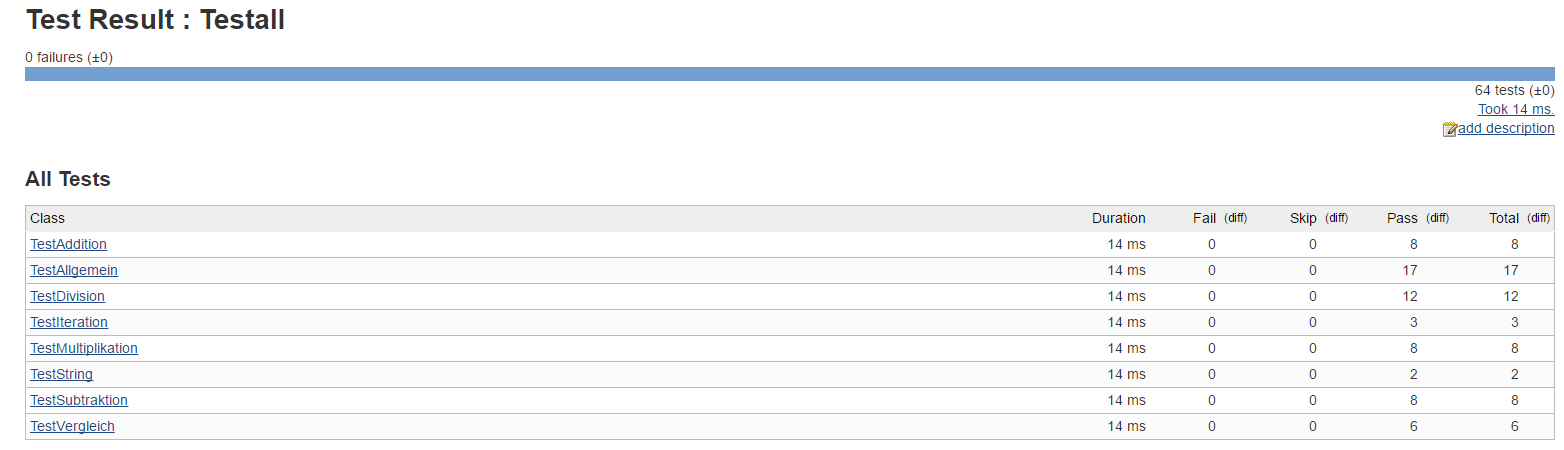
\includegraphics[width=1\linewidth]{images/tests}
\end{minipage}

\subsubsection{Violations report}
Es wurde versucht einen Violations report zu erzeugen, welcher auch erzeugt wird im \verb|pylint.out| File.

Dieser wird jedoch im Build nicht angezeigt aus einem unerklärlichem Grund. 